\documentclass{article} % For LaTeX2e
% ICLR 2026 style as scaffold — swap to iclr2027_conference when the kit is released.
\usepackage{iclr2026_conference,times}

\usepackage{amsmath,amsfonts,amssymb}
\usepackage{booktabs}
\usepackage{graphicx}
\usepackage{algorithm}
\usepackage{algorithmic}
\usepackage{xcolor}
\usepackage{hyperref}
\usepackage{url}
\input{math_commands}

% TODO markers — grep \todo before submission; nothing pending ships silently.
\newcommand{\takeaway}[1]{\vspace{2pt}\noindent\colorbox{gray!12}{\parbox{0.98\linewidth}{\small\textbf{Takeaway:} #1}}\vspace{2pt}}
\newcommand{\method}{Online SDFT}
\newcommand{\todo}[1]{\textcolor{red}{[TODO: #1]}}

\title{Streaming Self-Improvement of Language Models\\via Online Self-Distillation from Verifiable Feedback}

\author{Anonymous authors\\
Paper under double-blind review}

\newcommand{\fix}{\marginpar{FIX}}
\newcommand{\new}{\marginpar{NEW}}

\iclrfinalcopy % camera-ready style for readable drafts; comment out for submission
\begin{document}

\maketitle

\begin{abstract}
Language models deployed as agents produce a continual stream of interactions
whose outcomes can often be verified automatically, yet this experience is
typically discarded: weights are frozen at deployment, and the model repeats
its mistakes. Existing approaches to learning from deployment experience
either accumulate it in external memory, leaving the model itself unchanged,
or optimize the sparse outcome reward with reinforcement learning, which is
difficult to stabilize on long, heterogeneous interaction streams. We propose
\method{} (online self-distillation fine-tuning), which converts each verified
success into a weight update as it occurs. Concretely, verified outputs are
stored in a retrieval memory; the frozen base model, conditioned on a
problem's own verified answer as a hint, then serves as a teacher for the
deployed model, and its hint-conditioned token distribution is distilled into
LoRA adapters with a forward KL objective. The method requires no ground-truth
labels, no stronger teacher model, and no feedback beyond binary verification.
\method{} attains the best score on all seven StreamBench tasks, outperforming
retrieval-based in-context learning and REINFORCE-style baselines. On a fused
stream of 4{,}219 problems spanning three domains, a single continually
trained model outperforms three per-domain specialist models ($+3.4$ points on
code generation), whereas REINFORCE++ collapses under the induced distribution
shift. Moreover, at matched data and oracle budget, single-pass online updates
outperform multi-epoch offline training on the same experience. These results
suggest that verified deployment experience can serve directly as supervision
for continual model improvement.
\end{abstract}

\section{Introduction}
\label{sec:intro}

\begin{figure}[t]
\centering
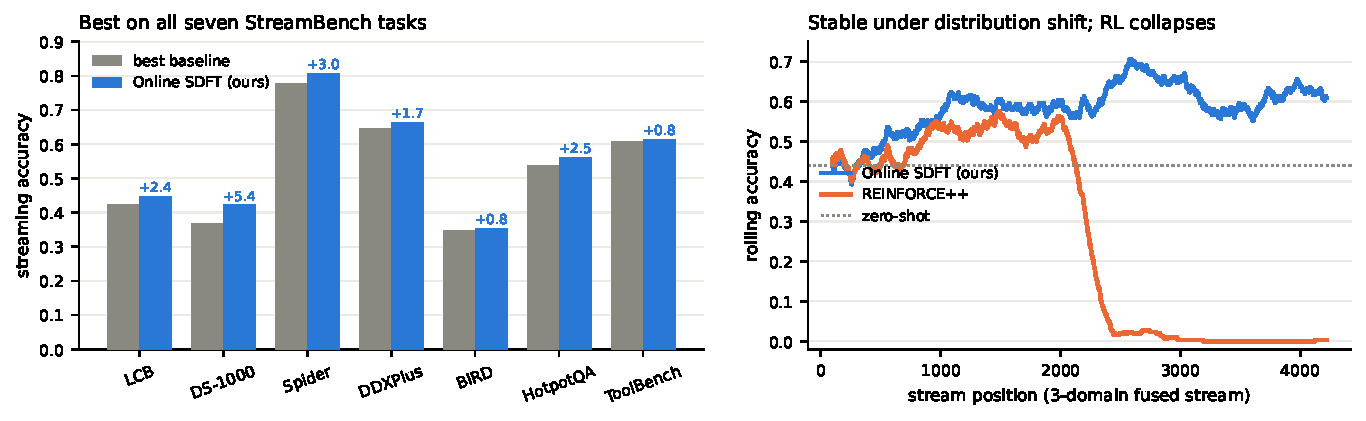
\includegraphics[width=\linewidth]{figures/fig1.pdf}
\caption{\textbf{Left:} final streaming accuracy on seven StreamBench tasks;
\method{} (blue) exceeds the strongest baseline (zero-shot, Self-StreamICL, or
REINFORCE++, gray) on every task. \textbf{Right:} rolling accuracy on a
4{,}219-problem stream interleaving three domains; \method{} improves throughout
while REINFORCE++ collapses after roughly 2{,}000 problems.}
\label{fig:headline}
\end{figure}

A language model deployed as an agent meets its work as a stream. A coding
assistant sees one issue after another, and each resolved ticket reveals whether
its patch passed the tests. The feedback is sparse, a single verified bit per
attempt, but it is grounded and it arrives continuously. Deployed models are
nevertheless frozen: a mistake made on Monday is repeated on Friday, because
nothing connects the stream of verified outcomes back to the weights.

Two research programs address parts of this problem. The first improves models
between deployments. Self-training methods sample from the model, keep outputs
that pass a correctness check, and fine-tune on the survivors
\citep{zelikman2022star, gulcehre2023rest, singh2024beyond, yuan2023scaling};
reinforcement learning from verifiable rewards scales the same signal to
emergent reasoning \citep{shao2024deepseekmath, guo2025deepseekr1}. These loops
need the task corpus up front and make several generation and training sweeps
over it, so they cannot run while the stream is being served. The second
program adapts agents during deployment but avoids weight updates: verified
experiences go into buffers, skill libraries, and playbooks that are retrieved
into the prompt \citep{shinn2023reflexion, wang2024voyager, zhao2024expel,
wang2025agent, madaan2022memprompt, zhang2025agentic}, the design StreamBench
\citep{wu2024streambench} adopted for streaming evaluation. Under this design
the model itself never improves. Gains are capped by the frozen base, disappear
without the memory, and retrieval can hurt when neighbors mislead
(\S\ref{sec:exp-bench}). Test-time training does update weights but discards
them after each instance \citep{sun2020ttt, akyurek2025surprising,
hubotter2025sift}. Applying rollout-batch RL to the streaming bit is also
problematic: policy-gradient methods are prone to entropy collapse on long
horizons even offline \citep{cui2025entropy, liu2025prorl}, and in our
experiments a stability-oriented variant \citep{hu2025reinforcepp} diverges on
a long mixed-domain stream.

What is missing is a stable online learning rule that turns each verified
success into a permanent weight update at the moment it happens. Our starting
point is a simple observation: \textbf{a model conditioned on its own
oracle-verified answer is a teacher for the same model without it.} Matching
the teacher's next-token distribution, with a forward KL against a frozen base
reference, moves the answer's information into the weights in a small and
verified step. We build \method{} around this rule. Verified answers enter a
reward-filtered memory \citep{wu2024streambench} that serves two purposes:
retrieval of demonstrations for the current problem, and hints for
distillation. Because a single greedy pass would only ever train on problems
the model already solves, a forward re-evaluation step retries recent failures
with the current model, which converts weight gains into new verified data.
Scoring always precedes any use of a problem for training, so the streaming
metric remains strictly predict-then-train.

We evaluate on seven StreamBench tasks and two stress tests.
\begin{itemize}
\item \textbf{Streaming accuracy} (\S\ref{sec:exp-bench}): \method{} reaches
  the best accuracy on all seven tasks against zero-shot, Self-StreamICL, and
  REINFORCE++ baselines, including tasks where retrieval-ICL falls below
  zero-shot.
\item \textbf{Distribution shift} (\S\ref{sec:exp-fused}): on a 4{,}219-problem
  stream interleaving three domains, one \method{} model matches or beats three
  per-domain specialists, with a $+3.4$-point gain on code relative to its own
  specialist. Retrieval stays within-domain for 99.9\% of queries, so this
  transfer is carried by the weights. REINFORCE++ diverges after roughly
  2{,}000 problems on the same stream.
\item \textbf{Online vs.\ batch} (\S\ref{sec:exp-transfer}): with loss, data,
  model, and oracle budget held fixed, streaming training beats batch
  self-distillation on source mastery; an exploration-augmented batch variant
  narrows the gap, isolating coverage as the main mechanism
  \todo{and transfer to an unseen domain as the remaining open comparison
  (runs in progress)}.
\item \textbf{Ablations} (\S\ref{sec:exp-ablations}): the gains are not
  explained by oracle budget, hint-conditioned generation, or sample count.
\end{itemize}
We are not aware of prior work that performs verified, weight-updating
self-distillation online over a deployment stream. The closest neighbors are
SDPO, which uses self-distillation inside rollout-batch RL \citep{hue2026sdpo};
offline SDFT, which requires a gold dataset \citep{yang2024selfdistillation};
and test-time methods whose updates are transient \citep{akyurek2025surprising}
or driven by unverified consensus rewards \citep{zuo2025ttrl}. Code,
per-problem logs, and a causal-ordering leakage audit are released.

\section{Problem Formulation}
\label{sec:formulation}

\paragraph{Streaming setting.} Following the online evaluation protocol of
StreamBench \citep{wu2024streambench}, an agent faces an input--feedback sequence
$(x_1, fb_1), (x_2, fb_2), \dots, (x_T, fb_T)$ drawn from a task distribution and
presented in a fixed, seeded order. At step $t$ the agent produces
\begin{equation}
\hat y_t \;=\; f\!\big(p(x_t,\, r(M_t)) \,\big|\, \theta_t\big),
\end{equation}
where $\theta_t$ are the current model weights, $M_t$ is an external memory,
$r(\cdot)$ a retriever, and $p(\cdot)$ a prompting template. The environment
returns \emph{binary verifiable feedback}
$fb_t = g(x_t, \hat y_t) \in \{0, 1\}$---execution of generated code against unit
tests, execution-match of SQL, exact/label match for QA and diagnosis. Gold
references exist only inside $g$; the agent observes the bit. After feedback, the
agent may update any of $(p, r, M, \theta)$; the methods we study differ precisely
in \emph{which} of these they update (Table~\ref{tab:taxonomy}).

\paragraph{Evaluation.} Performance is \emph{prequential}: $\hat y_t$ is produced
and scored before $x_t$ influences any component, and the stream is consumed once.
We report final cumulative accuracy
$\mathrm{Acc}_T = \tfrac{1}{T}\sum_{t=1}^{T} h(\hat y_t, y_t)$
(each task's native metric $h$) and, equivalently, cumulative regret
$R_T = \sum_{t=1}^{T} (1 - h(\hat y_t, y_t))$, which penalizes late learning.
All methods on a given task see the identical stream order.

\paragraph{Why this setting is hard.} The agent gets one attempt per problem, a
single bit per attempt, no gold text ever, and no second pass over the stream.
Improvements must therefore be bootstrapped from the agent's \emph{own} verified
outputs---and any weight update risks destabilizing performance on the remainder
of the stream, a risk realized dramatically by the RL baseline in
\S\ref{sec:exp-fused}.

\begin{table}[t]
\centering
\caption{Method taxonomy: what each method updates and what signal it consumes.
\method{} is the only method that both updates weights and exploits a dense,
token-level training signal derived from verified self-generated text.}
\label{tab:taxonomy}
\small
\begin{tabular}{lcccc}
\toprule
Method & Updates $M$ & Updates $\theta$ & Training signal & Signal density \\
\midrule
Zero-shot (Base) & -- & -- & -- & -- \\
Self-StreamICL & \checkmark & -- & -- (retrieval only) & -- \\
REINFORCE++ & -- & \checkmark & scalar reward & per sequence \\
\textbf{\method{} (ours)} & \checkmark & \checkmark & verified self-output & per token \\
\bottomrule
\end{tabular}
\end{table}

\section{Method: Online Self-Distillation from Verifiable Feedback}
\label{sec:method}

\paragraph{Setting.} Problems $x_1, x_2, \dots$ arrive in a fixed stream in
batches of $B{=}10$. For each problem the environment provides a binary oracle
$r(x, y) \in \{0, 1\}$ (test execution, exact match, label equality). Gold answers
exist only \emph{inside} the oracle; only the bit leaves it. The streaming metric
is prequential: every problem is answered and scored \emph{before} any update that
involves it. We maintain a policy $\pi_\theta$ (base model + LoRA), a frozen copy
of the base model $\pi_{\text{ref}}$, and a memory
$M : x \mapsto (y^\star, e)$ storing each problem's latest \emph{verified} answer
and an embedding of its question.

\paragraph{Per-batch loop.} Each stream batch triggers three phases
(Algorithm~\ref{alg:method}):

\textbf{(1) Score.} For each new $x$: retrieve the $k{=}3$ nearest past problems
from $M$ (embedding $k$NN, excluding $x$) as in-context demonstrations, generate
greedily, and query the oracle. The result is recorded---permanently---and, if
correct, the answer is stored in $M$ (reward filter).

\textbf{(2) Forward re-evaluation.} Problems from the last $W{=}9$ batches are
re-answered with the \emph{current} model and re-scored. Successes update $M$:
failures recovered by the improved model enter memory late, and existing entries
are refreshed into the current model's phrasing (keeping distillation targets
near on-policy). Re-evaluation never touches recorded scores.

\textbf{(3) Self-distillation.} For each window problem $x$ with $M(x) = y^\star$:
the \emph{student} sees prompt $P(x)$ = system + demos + $x$; the \emph{teacher}
sees $P(x)$ followed by $y^\star$ as an assistant turn and $x$ repeated. A
completion $\hat y$ is generated from the teacher prefix, and we minimize the
token-level forward KL
\begin{equation}
\mathcal{L}(\theta) \;=\; \sum_t \mathrm{KL}\!\left(
  \pi_{\text{ref}}(\cdot \mid P^{+}(x), \hat y_{<t}) \;\big\|\;
  \pi_\theta(\cdot \mid P(x), \hat y_{<t}) \right),
\label{eq:kl}
\end{equation}
where $P^{+}$ denotes the hint-augmented prompt. The teacher is the \emph{frozen
base} model---the only asymmetry is the hint. The student learns to produce the
teacher's hint-informed distribution \emph{without} the hint, compressing the
verified answer into the weights. We use 2 epochs per window pool, LoRA
($r{=}16$, $\alpha{=}32$, all linear layers), learning rate $5{\times}10^{-5}$,
and skip the first 3 completion tokens.

\paragraph{Why no leakage.} The hint is always the model's own earlier
oracle-passing output, never a dataset field; demos always come from strictly
earlier batches; and a problem's score is final before it can enter $M$. We audit
these causal-ordering invariants programmatically over the actual run logs
(Appendix~\ref{app:leakage}).

\paragraph{Generation source.} Conditioning the generated completion $\hat y$ on
the hint (vs.\ sampling it from the bare student prompt, as in offline
self-distillation) turns out to be a minor, bootstrap-phase choice: the two
settings differ by ${\sim}1$ point and only early in the stream
(\S\ref{sec:exp-ablations}), so our results do not hinge on it.

\begin{algorithm}[t]
\caption{Online SDFT (one stream batch)}
\label{alg:method}
\begin{algorithmic}[1]
\FOR{each new problem $x$ in batch $B_t$}
  \STATE $y \leftarrow \pi_\theta(\,\text{system} + \text{kNN}_3(M, x) + x\,)$ \hfill (greedy)
  \STATE record $r(x,y)$ \hfill (prequential metric; final)
  \IF{$r(x,y)=1$} \STATE $M[x] \leftarrow y$ \ENDIF
\ENDFOR
\FOR{each $x$ in last $W$ batches}
  \STATE $y' \leftarrow \pi_\theta(\,\text{system} + \text{kNN}_3(M, x) + x\,)$
  \IF{$r(x,y')=1$} \STATE $M[x] \leftarrow y'$ \hfill (recover / refresh) \ENDIF
\ENDFOR
\FOR{each $x$ in window pool with $M[x]=y^\star$}
  \STATE $\hat y \sim \pi_\theta(P^{+}(x))$;\quad update $\theta$ by Eq.~\ref{eq:kl}
\ENDFOR
\end{algorithmic}
\end{algorithm}

\section{Experiments}
\label{sec:exp}

\paragraph{Common setup.} All experiments use Qwen2.5-Coder-7B-Instruct with LoRA
($r{=}16$), greedy decoding, batch size 10, window $W{=}9$, $k$NN $k{=}3$
(Qwen3-Embedding-0.6B), seed-42 stream order identical across methods. Baselines:
\textbf{Base} (zero-shot, no adaptation), \textbf{ICL} (Self-StreamICL: reward-filtered
memory + $k$NN demos, frozen weights), and \textbf{REINFORCE++} (policy gradient with
global-whitened advantages, PPO clipping, KL to the frozen base, replaying stored
completions over the same rolling window). All methods see identical problems in
identical order; base, ICL, and REINFORCE++ use exactly one oracle call per problem
(cost accounting for SDFT in \S\ref{sec:exp-ablations}).

\subsection{Seven streaming benchmarks}
\label{sec:exp-bench}

Table~\ref{tab:bench} reports each benchmark's native accuracy over its full
stream. \textbf{Our method attains the best accuracy on all seven tasks}, spanning
competitive code generation, data-science code, two text-to-SQL tasks, medical
diagnosis, multi-hop QA, and function calling. Two patterns recur. First, ICL is a
strong baseline where retrieval finds near-duplicates (DDXPlus) but can
\emph{hurt} on tasks where retrieved demonstrations mislead (HotpotQA: $0.509$ vs
base $0.521$); self-distillation recovers and surpasses base in exactly those
cases ($0.562$), because the signal is consolidated in weights rather than
recalled at inference. Second, REINFORCE++ is inconsistent---above ICL on some
tasks, far below base on others (Spider $0.587$ vs $0.747$)---previewing the
stability failure of \S\ref{sec:exp-fused}.

\begin{table}[t]
\centering
\caption{Streaming accuracy on seven StreamBench tasks (native metric per task;
identical stream order and model for all methods). Our method is best on all
seven.}
\label{tab:bench}
\begin{tabular}{llrrrrr}
\toprule
Benchmark & Domain & Size & Base & ICL & R++ & \textbf{Ours} \\
\midrule
LiveCodeBench & code & 1055 & 0.338 & 0.424 & 0.386 & \textbf{0.448} \\
DS-1000 & Python & 955 & 0.325 & 0.367 & 0.369 & \textbf{0.423} \\
Spider & text-to-SQL & 2147 & 0.747 & 0.778 & 0.587 & \textbf{0.808} \\
DDXPlus & medical dx & 1764 & 0.436 & 0.647 & 0.404 & \textbf{0.664} \\
BIRD & hard SQL & 1534 & 0.330 & 0.346 & 0.271 & \textbf{0.354} \\
HotpotQA & multi-hop QA & 1500 & 0.521 & 0.509 & 0.537 & \textbf{0.562} \\
ToolBench & func-calling & 750 & 0.549 & 0.593 & 0.607 & \textbf{0.615} \\
\bottomrule
\end{tabular}

\end{table}

\subsection{Distribution shift: one model, three domains}
\label{sec:exp-fused}

We interleave DS-1000 (code, 955), DDXPlus (diagnosis, 1{,}764), and HotpotQA
(QA, 1{,}500) into a single 4{,}219-problem stream by a random merge that
\emph{preserves each domain's internal order}, making per-domain slices exactly
comparable to the standalone runs. Table~\ref{tab:fused} shows the outcome.

\begin{table}[t]
\centering
\caption{Fused-stream results (4{,}219 problems). ``SDFT standalone'' aggregates
the three per-domain runs at matched prefixes (regret summed, accuracy weighted).
One online-distilled model matches or beats three specialists.}
\label{tab:fused}
\begin{tabular}{lrrrrr}
\toprule
Method & Acc & Cum.\ regret & DS-1000 & DDXPlus & HotpotQA \\
\midrule
Base & 0.439 & 2365 & 0.318 & 0.436 & 0.521 \\
ICL $k{=}3$ & 0.533 & 1971 & 0.358 & 0.647 & 0.509 \\
REINFORCE++ (fused) & 0.253 & 3153 & 0.213 & 0.262 & 0.267 \\
SDFT standalone ($3\times$) & 0.573 & 1800 & 0.423 & 0.664 & \textbf{0.562} \\
\textbf{SDFT fused (ours)} & \textbf{0.585} & \textbf{1750} & \textbf{0.457} & \textbf{0.676} & 0.560 \\
\bottomrule
\end{tabular}

\end{table}

Three findings. \textbf{(i) One model $\geq$ three specialists:} the fused model
beats the aggregated standalone runs overall ($.585$ vs $.573$) and is no worse on
any domain, with \emph{positive} cross-domain transfer to code ($+3.4$ points on
DS-1000). \textbf{(ii) Transfer lives in the weights:} retrieval self-segregates
---99.9\% of retrieved demonstrations are same-domain (2 of 2{,}059 queries pull
any cross-domain demo)---so prompts are effectively domain-pure and cannot explain
the gains. \textbf{(iii) RL collapses:} REINFORCE++ tracks ${\sim}5$ points below
SDFT for 2{,}000 problems, then diverges catastrophically (approximate KL turns
negative, clip fraction spikes $0.08{\to}0.68$, advantage std triples); accuracy
falls to zero for the remainder of the stream (final $0.253$). The same
hyperparameters are stable on every shorter standalone stream, indicating a
long-horizon instability that online self-distillation simply does not exhibit:
its per-window KL objective is anchored to a frozen teacher and its rolling
accuracy climbs monotonically ($.44 \to .68$ peak) over the same stream
(Figure~\ref{fig:trend}).

\begin{figure}[t]
\centering
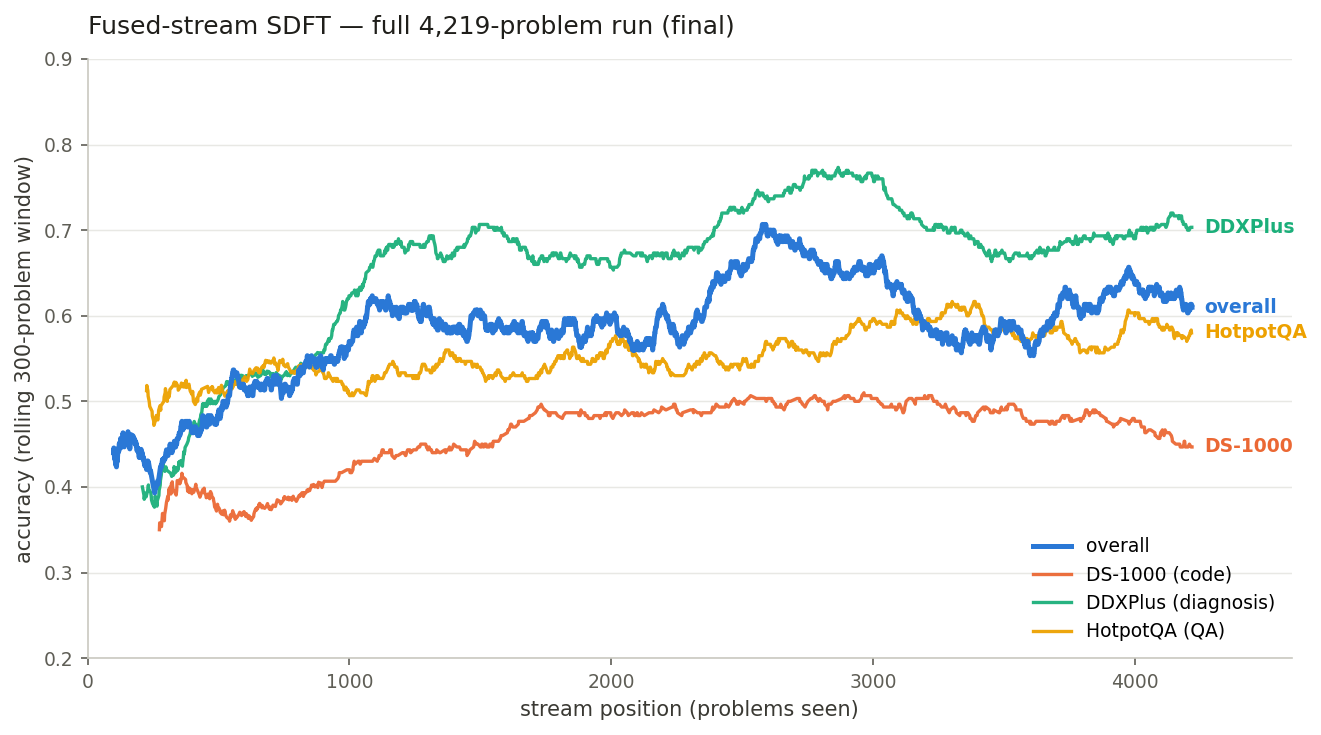
\includegraphics[width=0.9\linewidth]{figures/fused_accuracy_trend.png}
\caption{Rolling accuracy (300-problem window) of online SDFT over the fused
three-domain stream, overall and per domain. All domains improve simultaneously;
no interference from distribution shift.}
\label{fig:trend}
\end{figure}

\subsection{Online vs.\ batch training}
\label{sec:exp-transfer}

Does the \emph{online schedule itself} matter, beyond the loss? We compare our
online run on DS-1000 against \emph{batch} self-distillation: the identical
trainer, loss, model, and oracle, but run as classic offline epochs (4 passes over
all 955 problems; per pass: generate, oracle-filter, distill on verified answers;
no memory, no stream). We then evaluate both resulting adapters with a single
bare-prompt greedy pass over the full problem set (no demonstrations, no memory).

\begin{table}[h]
\centering
\caption{Source-data mastery after training on DS-1000 (bare-prompt greedy pass,
all 955 problems).}
\label{tab:mastery}
\begin{tabular}{lrr}
\toprule
Model & Acc & Solved / 955 \\
\midrule
Base & 0.313 & 313 \\
Batch SDFT (4 epochs) & 0.425 & 406 \\
\textbf{Online SDFT (ours)} & \textbf{0.480} & \textbf{458} \\
\bottomrule
\end{tabular}

\end{table}

The online-trained model solves $458/955$ ($.480$) versus $406$ ($.425$) for
batch---a $+5.5$-point gap \emph{on the very data batch trained on for four
epochs}---and its advantage comes from breadth: 123 problems only online solves vs
71 only batch solves, with equal (small) forgetting relative to base. We attribute
the gap to the stream's implicit curriculum: each problem is revisited across a
rolling window while the model evolves, and forward re-evaluation keeps
converting newly in-reach problems into training signal, whereas single-sample
batch generation can only ever train on what the current model already solves.
\todo{Batch with $n{=}5$ sampled attempts per problem (running) tests whether
exploration closes this gap.}
\todo{Transfer: both adapters warm-start online SDFT on the unseen HotpotQA
stream; compare accuracy/regret vs from-scratch ($.562$/657). Runs pending.}

\subsection{Ablations and cost}
\label{sec:exp-ablations}

\textbf{Generation source.} Sampling the distillation completion from the bare
student prompt (offline-SDFT default) vs the hint-conditioned prefix (ours)
changes DS-1000 by $+1.3$ points in favor of the former, with the difference
confined to the early stream; on the fused stream the two are even after a small
early deficit. The choice is a bootstrap-phase detail, not a driver.
\textbf{Epochs.} 4 inner epochs beat 2 on DS-1000 ($+21$ cumulative-regret at
matched pressure); learning-rate increases do not substitute for epochs.
\textbf{Multi-sample distillation.} Distilling from $N{=}10$ sampled candidates
(filtered or not) matches single-sample distillation---sample \emph{count} is not
the bottleneck.
\textbf{Oracle budget.} Our method issues ${\sim}9.8$ oracle calls per problem
(1 scored on arrival + ${\sim}8.8$ memory-only re-evaluations); baselines use 1.
The extra calls only gate memory; they never alter recorded scores. Giving ICL
the same budget would not help---a frozen model re-answering with the same
distribution recovers almost nothing---and REINFORCE++ at 1 call/problem already
shows that training-with-feedback alone does not close the gap.

\section{Analysis: Why Online Self-Distillation Works}
\label{sec:analysis}

\paragraph{The flywheel.} The method's components are individually simple but
mutually reinforcing: weight updates improve the model; forward re-evaluation lets
the improved model recover problems it failed on arrival ($84$ of $1{,}463$
memory entries in the fused run entered late this way); recovered problems become
demonstrations and distillation targets; and fresher targets keep the KL objective
near on-policy. A frozen-weights method (ICL) receives none of this---re-answering
with an unchanged model recovers almost nothing---and pure RL receives the reward
but not the dense token-level signal.

\paragraph{Distillation as supervision, memory as scaffolding.} Wherever ICL
hurts (HotpotQA, misleading neighbors), self-distillation still helps: the hint
channel injects only the model's own \emph{verified} answer for the \emph{same}
problem, a signal that cannot mislead. Conversely, wherever ICL is strong
(DDXPlus), consolidation into weights preserves the gains while freeing the
context window.

\paragraph{Stability.} The distillation loss (Eq.~\ref{eq:kl}) is anchored to a
frozen reference teacher and its targets are always oracle-verified text. There
is no advantage estimate, no clipped ratio, no moving critic---the failure
surfaces that destroyed REINFORCE++ on the long fused stream simply do not exist.
Across ${\sim}12{,}000$ streamed problems in this paper, online SDFT never
regressed catastrophically.

\paragraph{Predict-then-train integrity.} Because every reported number is
produced by a model that had never seen that problem---scored before storage,
demonstrations strictly from the past, hints strictly self-generated---the
streaming metric doubles as a continual-generalization measure. We release a
causal-ordering audit that verifies these invariants over the raw run logs
(Appendix~\ref{app:leakage}).

\section{Related Work}
\label{sec:related}

\paragraph{Streaming adaptation and memory-based improvement.}
StreamBench \citep{wu2024streambench} formalizes online LLM improvement under
prequential evaluation with binary feedback and shows that
\emph{Self-StreamICL}---storing only verified-correct self-outputs and retrieving
them as demonstrations---is the strongest single-agent streaming strategy,
with the correctness filter being essential (storing incorrect outputs, even
labeled as such, does not help). Our ICL baseline is exactly this method, and
our memory inherits its filter. MemPrompt \citep{madaan2022memprompt} pioneered
deployment-time memory of user feedback for prompt editing; reflection-style
agents \citep{shinn2023reflexion} accumulate verbal self-critiques. All of
these adapt the \emph{context}; the model itself never improves, gains are
bounded by the frozen model's ability, and they vanish without the memory. Our
mastery evaluation (\S\ref{sec:exp-transfer}) makes this limitation concrete,
and our method converts the same filtered memory into permanent weight gains.

\paragraph{Self-distillation and distillation from self-generated data.}
Offline SDFT \citep{yang2024selfdistillation} shows that fine-tuning on the
model's \emph{own} rewrites of gold answers---rather than the gold text
itself---preserves general capabilities by keeping training targets inside the
model's output distribution; their mix-ratio analysis ties forgetting causally
to target-distribution shift. Generalized knowledge distillation
\citep{agarwal2024gkd} distills on-policy student samples against a teacher's
distribution. SDPO \citep{hue2026sdpo} makes the model conditioned on
environment feedback a \emph{self-teacher} inside policy optimization, showing
the resulting gradient is a policy gradient with dense logit-level advantages,
with strong results on rollout-batch RL for code. Our method transplants the
self-teacher idea to the \emph{streaming} setting: the conditioning signal is a
verified answer harvested online from the model's own past, the loss is anchored
to a frozen reference (no moving teacher), and the surrounding machinery
(reward-filtered memory, forward re-evaluation) exists precisely to keep minting
such answers from a single pass over the data. Where SDPO and GKD are
offline/rollout-batch, we show the online schedule is itself a source of
gains (\S\ref{sec:exp-transfer}).

\paragraph{Reinforcement learning from verifiable rewards.}
GRPO \citep{shao2024deepseekmath}, RLOO \citep{ahmadian2024rloo}, and
REINFORCE++ \citep{hu2025reinforcepp} optimize scalar verifiable rewards and
power modern reasoning models. The scalar signal is thin---one bit per
attempt---and credit assignment is per-sequence. Our experiments show a faithful
REINFORCE++ under the identical streaming skeleton is unstable on long
heterogeneous streams (\S\ref{sec:exp-fused}); self-distillation extracts a
per-token signal from the same oracle bit and remains stable.

\paragraph{Continual learning and test-time training.}
Our setting is continual learning without task boundaries
\citep{parisi2019continual}, sharing its central tension between plasticity and
stability, but with verifiable feedback in place of supervised labels; the fused
experiment is a task-incremental stress test in which our method exhibits
transfer rather than interference. Test-time training \citep{sun2020ttt} adapts
per-instance and discards the update; our updates are cumulative and permanent.
Self-improvement via self-training on filtered generations
\citep{zelikman2022star, gulcehre2023rest} is the offline, multi-epoch
ancestor of our per-window updates---our online-vs-batch comparison
(\S\ref{sec:exp-transfer}) isolates exactly what the streaming schedule adds
over that recipe.

\section{Discussion, Limitations, and Conclusion}
\label{sec:conclusion}

\paragraph{Discussion.} Our results argue that the two prevailing programs for
deployment-time improvement---accumulating experience outside the model and
optimizing the scalar feedback bit with policy gradients---leave value on the
table that a third route captures: internalizing each verified experience into
the weights through anchored self-distillation. The streaming schedule is not an
obstacle to engineer around but an asset: it supplies an emergent curriculum and
a data flywheel that batch training on the same data cannot reproduce.

\paragraph{Limitations.} Our experiments use a single 7B code-centric model with
LoRA adapters and one stream order per task (StreamBench's released sequences);
multi-seed variance is not characterized. Feedback is binary---richer textual
feedback \citep{hue2026sdpo} is unexplored in our setting. Our method spends
${\sim}10\times$ more oracle calls than the baselines (on memory maintenance,
not scoring), a real cost where verification is expensive. General-capability
retention beyond the streamed tasks (e.g., on knowledge benchmarks) is not yet
measured. \todo{Transfer-to-unseen-domain runs and the exploration-matched batch
arm are pending.}

\paragraph{Conclusion.} We presented \method{}, to our knowledge the first
method to perform verified, weight-updating self-distillation online over a
deployment stream: verified self-generated answers feed a reward-filtered
memory that serves retrieval today and distillation forever, with forward
re-evaluation converting weight gains back into training data. \method{} is
best on all seven StreamBench tasks, absorbs a three-domain distribution shift
that collapses a stability-engineered RL baseline---with one model beating
per-domain specialists through weight-borne transfer---and outperforms batch
training with the identical objective on identical data. Deployed models need
not be frozen: a single pass of grounded feedback is enough to learn from.

\subsection*{Reproducibility Statement}
All benchmarks are public (StreamBench and its constituent datasets;
Table~\ref{tab:datasets} lists sources), and all methods use an open-weights
model (Qwen2.5-Coder-7B-Instruct) with fixed released stream orders (seed 42),
making every run exactly repeatable. Complete hyperparameters appear in
Appendix~\ref{app:hparams}, prompt templates in Appendix~\ref{app:prompts}, and
oracle definitions in \S\ref{sec:exp-setup}. Our released repository contains
all training and evaluation code, per-problem logs for every run in every
table, the table-generation scripts that produce the paper's numbers directly
from those logs, and the causal-ordering audit of Appendix~\ref{app:leakage}.


\bibliography{refs}
\bibliographystyle{iclr2026_conference}

\appendix
\section{Leakage Audit}
\label{app:leakage}
We verify four causal-ordering invariants programmatically over the raw run logs
of the fused experiment (script released with the code): (A) every problem is
scored exactly once; (B) no memory entry predates its problem's scoring batch;
(C) memory is append-only with respect to the stream, so retrieved demonstrations
always come from strictly earlier batches; (D) aggregate counters match the
per-problem log. All checks pass. Gold labels exist only inside the 0/1 oracle;
the stored hint is always the model's own earlier oracle-passing output.
\todo{Include example student/teacher prompt traces (available in the repo's
leakage-audit folder).}

\section{Hyperparameters and Reproducibility}
\label{app:hparams}
\todo{Full hyperparameter table (LoRA config, lengths, decoding, trainer
settings), hardware (single H200 per run), and per-benchmark oracle definitions.
All code, per-problem CSVs, and analysis scripts are in the released repository.}

\section{Additional Ablations}
\label{app:ablations}
\todo{Full ablation tables: generate-from-teacher (standalone + fused),
epoch/learning-rate grid, multi-sample distillation (filtered and unfiltered
$N{=}10$), REINFORCE++ collapse diagnostics (KL/clip-fraction/advantage-std
trajectories).}


\end{document}
